\documentclass[11pt,a4paper]{article}
\usepackage[T1]{fontenc}
\usepackage[utf8]{inputenc}
\usepackage[french]{babel}
\usepackage{lmodern}
\usepackage{amsmath,amssymb}
\usepackage[margin=2.35cm]{geometry}
\usepackage{booktabs,longtable,tabularx}
\usepackage{enumitem}
\usepackage{graphicx}
\usepackage{xcolor}
\usepackage{microtype}
\usepackage{float}
\usepackage{hyperref}

\hypersetup{colorlinks=true,linkcolor=blue!45!black,urlcolor=blue!45!black}
\setlist{nosep}
\newcommand{\code}[1]{\texttt{#1}}
\newcommand{\Kaut}{K^{*}_{\mathrm{aut}}}
\newcommand{\fait}{\textbf{[Fait observé]}}
\newcommand{\inference}{\textbf{[Inférence]}}
\newcommand{\hyp}{\textbf{[Hypothèse]}}
\newcommand{\incertitude}{\textbf{[Incertitude]}}

\title{M4.2B --- rapport final\\
\large Émergence et contrôle d'une queue Pareto des revenus d'intérêt,
sous contrainte de cascades critiques}
\author{Programme M4.2B --- dossier \code{m4\_2b\_credit\_soc}}
\date{6 août 2026}

\begin{document}
\maketitle

\begin{abstract}
Ce document synthétise l'ensemble du programme M4.2B --- phase pilote
(30 juillet), campagne d'exploration (87 runs, 29 cellules $\times$ 3
graines), campagne de confirmation (45 runs, 9 cellules $\times$ 5
graines \textbf{disjointes}, jamais vues avant).

\textbf{Résultat central} : trois versions successives d'un test
d'existence d'une queue de Pareto robuste (stabilité de l'exposant
$\hat\alpha$ au changement de seuil) ont été tentées sur les 37
cellules du programme ; aucune n'a pu trancher, ni dans un sens ni dans
l'autre (\S\ref{sec:criteres}). La dernière (facteur d'admissibilité
continu, bootstrap sur 132 runs) montre que le facteur limitant est
presque partout le \textbf{volume de données disponible dans la queue
extrême}, pas une preuve de courbure. \textbf{Décision} (6 août 2026) :
l'existence de la queue de Pareto est posée comme \textbf{hypothèse de
travail}, en reconnaissant explicitement le « coude » présent après la
cassure dans toutes les simulations de ce programme ; ce rapport
caractérise désormais $\hat\alpha$ et son incertitude plutôt que de
continuer à tester son existence. Sous cette hypothèse, $\hat\alpha$ est
reproductible d'une graine à l'autre (écart-type inter-graines médian
$0{,}070$, contre un écart-type intra-instantané médian $0{,}341$) et
répond de façon interprétable aux paramètres testés
(\S\ref{sec:parametres}) --- c'est ce résultat, positif et quantitatif,
qui constitue l'apport substantiel de ce rapport. L'indépendance de
taille de l'exposant d'avalanche (objectif B) n'est ni établie ni
testable avec la conception actuelle de la confirmation.
\end{abstract}

\tableofcontents

\section{Contexte : le programme M4.2B en deux phrases}

M4.2B est une simulation multi-agents d'une économie de crédit : des
entités abstraites empruntent, prêtent, se versent des intérêts, et
peuvent faire faillite --- une faillite pouvant en déclencher d'autres
en cascade (« avalanche »). Le programme poursuit deux objectifs
\textbf{simultanés} :

\begin{itemize}
\item \textbf{Objectif A} --- Le revenu d'intérêt réellement perçu par
  chaque entité à un instant donné a-t-il, dans une région significative
  de l'espace des paramètres, une distribution à queue épaisse de type
  \textbf{Pareto}, et cette queue peut-elle être pilotée de façon
  reproductible en agissant sur la structure du marché du crédit --- en
  particulier sur l'intensité des appariements emprunteur/prêteur
  (paramètre $\eta$, voir \S\ref{sec:reperes}) ?
\item \textbf{Objectif B} --- Quel que soit le réglage trouvé pour
  l'objectif A, il ne doit pas détruire une propriété déjà établie dans
  les versions antérieures du modèle : la taille des cascades de
  faillites suit une loi de puissance, signature d'une dynamique proche
  d'un point critique.
\end{itemize}

La modification constitutive de M4.2B (par rapport à M4.2) est la
\textbf{cible de principal arithmétique} : lors d'une rencontre entre un
prêteur de capital $K_\ell$ et un emprunteur de capital $K_b$
($K_\ell>K_b$), les deux capitaux sont ramenés exactement à leur moyenne
$(K_\ell+K_b)/2$ (contre une cible géométrique $\sqrt{K_\ell K_b}$ en
M4.2). Le taux d'intérêt lui-même est inchangé (moyenne géométrique des
rendements marginaux des deux parties).

\section{Méthode : trois phases, un budget de calcul croissant}

\begin{enumerate}
\item \textbf{Phase pilote} (30 juillet) : quelques dizaines de runs
  choisis à la main pour maximiser l'information causale (baseline,
  contrôle géométrique, balayages $\sigma$ et $\lambda$) avant tout
  engagement de calcul dans une grille exhaustive.
\item \textbf{Campagne d'exploration} : 29 combinaisons de paramètres
  (« cellules »), chacune sur 3 graines aléatoires (0, 1, 2), 3000 pas
  de temps simulés (une cellule à 10\,000 pas pour vérifier l'horizon
  long) --- 87 runs, tous terminés avec succès.
\item \textbf{Campagne de confirmation} : 9 cellules retenues d'après
  l'exploration, chacune sur \textbf{5 graines nouvelles} (10 à 14,
  jamais vues pendant l'exploration), mêmes critères numériques que ceux
  fixés \emph{avant} de lancer l'exploration --- 45 runs, tous terminés
  avec succès. C'est la confirmation, pas l'exploration, qui établit les
  résultats numériques de ce rapport quand une cellule y figure
  (\S\ref{sec:resultat}).
\end{enumerate}

\begin{table}[h]
\centering
\small
\begin{tabularx}{\textwidth}{@{}llX@{}}
\toprule
Cellule & Paramètre testé & Motif de sélection \\
\midrule
\code{rho\_0.125}, \code{rho\_4} & $\eta$ linéaire, extrêmes & effet le plus net sur tous les diagnostics \\
\code{K0\_1}, \code{K0\_2000} & $K_0$, extrêmes & branche prioritaire (mécanisme \emph{deg\_out}) \\
\code{gamma\_0.6667} & $\gamma$, effet net (brut) & cartographie de la concavité \\
\code{control\_geometric} & cible géométrique (M4.2) & comparaison institutionnelle (question 1) \\
\code{deltasigma\_0.1\_0.1} & $\delta=\sigma=0{,}10$ & seule cellule à sortir du bruit sur la stabilité de seuil \\
\code{gamma\_comp\_0.3333/0.6667} & $\gamma$, $K_0$ compensé & effet $\gamma$ le plus propre, échelle contrôlée \\
\bottomrule
\end{tabularx}
\caption{Les 9 cellules de confirmation. Détail complet du choix :
\code{report/selection\_confirmation.md}.}
\end{table}

\section{Repères : ce que mesurent les grandeurs citées plus loin}
\label{sec:reperes}

\begin{itemize}
\item \textbf{$K_0$} : le capital de départ d'une entité nouvellement créée.
\item \textbf{$\Kaut$} : le capital vers lequel une entité isolée
  convergerait naturellement à long terme (équations de
  production/dépréciation du modèle). Ce qui compte est le rapport
  $K_0/\Kaut$, pas la valeur brute de $K_0$.
\item \textbf{$\gamma$} : la concavité de la fonction de production.
  $\gamma$ petit = rendements fortement décroissants ; $\gamma$ proche de
  1 = rendements presque linéaires.
\item \textbf{$\eta$} : le nombre de tentatives d'appariement
  emprunteur/prêteur à chaque pas de temps. Famille \textbf{linéaire}
  (facteur $\rho$, $\rho=1$ = référence) et famille \textbf{non
  linéaire} (exposant $\beta$).
\item \textbf{$\delta$, $\sigma$} : $\delta$ = taux de dépréciation du
  capital par pas ; $\sigma$ = amplitude des chocs aléatoires
  individuels sur la production.
\item \textbf{$\lambda$} : contrôle la démographie/taille du système
  (non re-testé en exploration/confirmation, fixé à 30 partout --- seule
  évidence : le balayage du pilote, voir \S\ref{sec:limites}).
\item \textbf{$r$, $q$, $rq$} : $r$ = taux d'intérêt appliqué ; $q$ =
  montant remboursé par contrat ; $rq$ = service payé par contrat.
  Mécanisme établi en phase pilote : la dispersion du revenu d'intérêt
  entre entités se décompose en une part due au \textbf{nombre de
  contrats actifs accumulés} (\emph{deg\_out}, effet de quantité) et une
  part due à \textbf{$rq$ moyen par contrat} (effet de prix).
\item \textbf{$\hat\alpha$, seuil, et statut de l'hypothèse Pareto} :
  $\hat\alpha$ est l'exposant ajusté (maximum de vraisemblance) d'une
  loi de puissance sur la queue des revenus, au-delà d'un seuil
  sélectionné par minimisation de la distance de Kolmogorov-Smirnov
  (méthode Clauset-Shalizi-Newman). Ce rapport a d'abord tenté de
  \textbf{tester} l'existence d'une vraie queue de Pareto (stabilité de
  l'exposant quand le seuil varie) avant de conclure que ce test n'est
  pas calculable de façon fiable avec le volume de données disponible
  (\S\ref{sec:criteres}). \textbf{L'existence de la queue de Pareto est
  donc désormais posée comme hypothèse de travail, pas démontrée} ---
  toutes les valeurs de $\hat\alpha$ de ce rapport doivent être lues
  sous cette réserve. Un « coude » est par ailleurs présent après la
  cassure dans toutes les simulations (connu, pas testé formellement) :
  $\hat\alpha$ caractérise la région immédiatement au-delà du seuil
  retenu, pas un comportement asymptotique à l'infini.
\item \textbf{Écart-type bootstrap de $\hat\alpha$} : puisque
  l'existence n'est plus testée, l'effort porte sur la
  \textbf{précision} de l'estimation de $\hat\alpha$. Trois échelles
  d'incertitude, gardées séparées (\S\ref{sec:criteres}) :
  \emph{intra-instantané} (rééchantillonnage bootstrap d'une seule coupe
  transversale, seuil re-sélectionné à chaque tirage),
  \emph{inter-instantanés} (dispersion de $\hat\alpha$ entre plusieurs
  instantanés d'un même run), \emph{inter-graines} (dispersion de la
  moyenne de run entre graines indépendantes d'une même cellule). Elles
  répondent à des questions différentes et ne sont jamais fusionnées en
  un seul nombre.
\item \textbf{$n_{\mathrm{tail}}$} : nombre de points utilisés pour
  l'ajustement de la queue.
\item \textbf{Test de Vuong} : compare deux modèles de distribution
  concurrents (loi de puissance contre exponentielle, ou contre
  lognormale) et indique lequel est mieux supporté par les données.
\item \textbf{$\hat\tau$ et rapport de branchement} : $\hat\tau$ =
  exposant de loi de puissance sur la taille des avalanches. Le rapport
  de branchement est le nombre moyen de faillites supplémentaires
  déclenchées par une faillite --- proche de 1 = dynamique de cascade
  proche d'un régime critique.
\item \textbf{Plancher de renouvellement} : fraction du décile le plus
  riche initial encore présente dans le décile le plus riche en fin de
  fenêtre. Proche de 0 = renouvellement total (grande mobilité) ; proche
  de 1 = élite figée.
\item \textbf{Indice de Gini($K$)} : mesure standard d'inégalité du
  capital entre entités (0 = parfaitement égal, 1 = concentration
  extrême).
\end{itemize}

\begin{figure}[H]
\centering
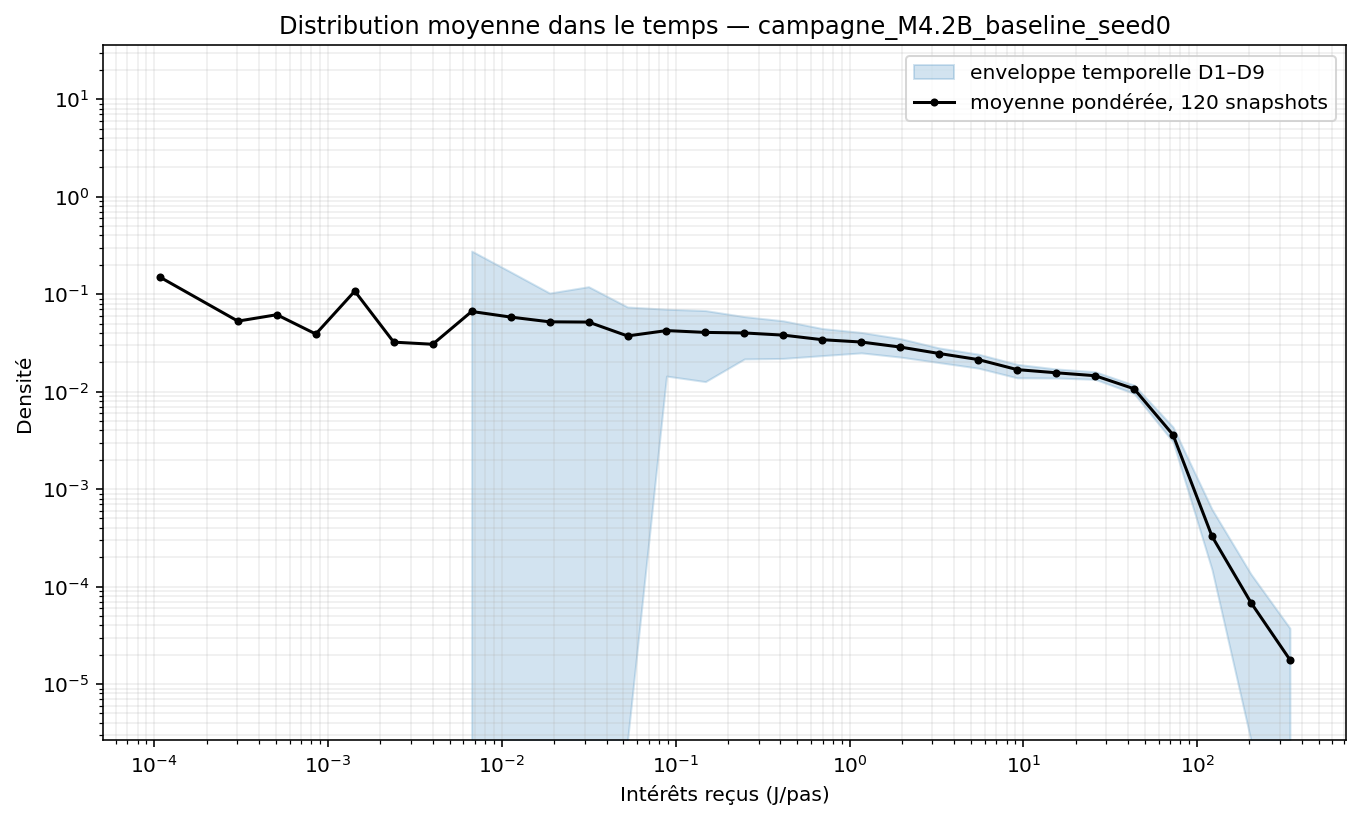
\includegraphics[width=0.72\textwidth]{figures/sim_interets_baseline.png}
\caption{Distribution moyenne dans le temps des intérêts reçus,
baseline ($\gamma=0{,}5$, $K_0=25$, $\delta=\sigma=0{,}01$), échelle
log-log. Sortie brute du moteur de simulation. Lecture : chaque point
est la densité moyenne, sur 120 instantanés, du montant d'intérêt reçu
par les entités actives à un instant donné. Une vraie loi de Pareto
apparaîtrait comme une droite sur la partie haute (à droite) ; ici la
courbe s'incurve et chute abruptement au-delà de $\sim$50 J/pas --- le
« coude » évoqué plus haut, présent dans toutes les simulations de ce
programme. C'est précisément ce qui a rendu le test d'existence
impossible à trancher (\S\ref{sec:criteres}) et qui motive de poser
l'existence de la queue de Pareto comme hypothèse plutôt que de
continuer à la tester.}
\end{figure}

\paragraph{Exemple travaillé --- comment le seuil est choisi et
comment $\hat\alpha$ et son incertitude bootstrap sont calculés.} La
figure ci-dessous applique le code de caractérisation
(\texttt{scripts/tail\_test.py}, \texttt{scripts/}
\texttt{admissibility\_factor.py}, sans aucune modification) à un
instantané réel : baseline, graine 0, pas $t=2225$ (choisi car son
$\hat\alpha$ est le plus proche de la moyenne des 91 instantanés
identifiables de ce run --- ni un cas particulièrement stable, ni
particulièrement instable).

\begin{figure}[H]
\centering
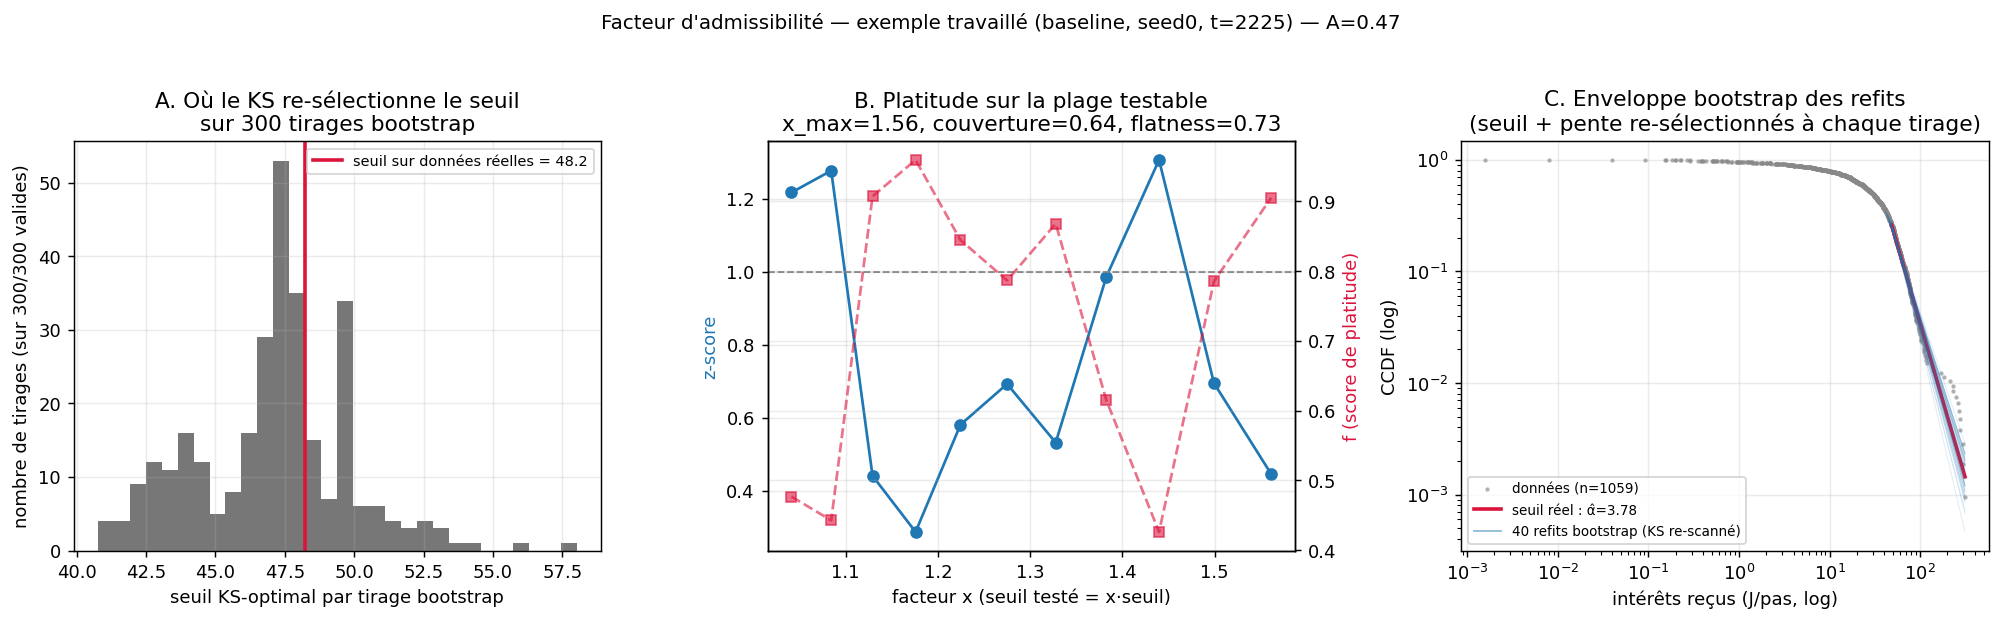
\includegraphics[width=0.95\textwidth]{figures/fig10_admissibilite_exemple.png}
\caption{Exemple travaillé : seuil, bootstrap et incertitude sur
$\hat\alpha$. Panneau A --- 300 tirages bootstrap (rééchantillonnage
avec remise, seuil KS \textbf{re-sélectionné à chaque tirage}) : la
distribution des seuils retrouvés est unimodale, centrée juste au-dessus
du seuil sur les données réelles (ligne rouge, 48,2) --- pas de second
mode qui indiquerait que le coude est parfois accroché à la place de la
vraie cassure sur cet instantané. C'est cette distribution qui donne
l'écart-type bootstrap de $\hat\alpha$ (intra-instantané) : $0{,}34$ en
moyenne sur les 129 runs caractérisés --- nettement plus large que la
dispersion entre graines (\S\ref{sec:resultat}). Panneau C ---
l'enveloppe des 40 refits bootstrap (seuil et pente re-sélectionnés à
chaque tirage) tracée directement sur la CCDF empirique : visualisation
directe de cette incertitude. Le panneau B (test de platitude par
facteur de seuil) est un diagnostic historique de la tentative de test
d'existence (\S\ref{sec:criteres}) --- gardé pour traçabilité, plus
utilisé comme critère.}
\end{figure}

\section{Du test d'existence à la caractérisation : ce qui a changé et pourquoi}
\label{sec:criteres}

\textbf{Ce qui a été tenté d'abord.} Le protocole pré-enregistré (avant
tout résultat de confirmation) définissait un test d'existence en 5
critères pour qualifier une queue de Pareto de « robuste » --- le
premier (stabilité de l'exposant $\hat\alpha$ quand le seuil varie)
s'est révélé être la condition qui bloque tout : sur les 45 runs de
confirmation, il échouait 0/5 graines, sur les 9 cellules, sans
exception. Deux révisions successives de ce critère ont été tentées :

\begin{enumerate}
\item \textbf{Seuil moitié vs seuil optimal} (version initiale du
  protocole) : rejetée après relecture --- ce test compare la queue au
  corps de la distribution (déjà modélisé séparément par GB2), pas la
  queue à elle-même ; il échoue quasiment par construction.
\item \textbf{Seuil $\times 2$ vs seuil optimal} (auto-similarité d'une
  vraie loi de puissance, la bonne idée) : recalculée sur les
  instantanés effectivement utilisables (\texttt{scripts/probe\_
  criterion1\_2x.py}) --- à seuil $\times 2$, le nombre de points de
  queue tombe de 113 (médiane) à 17, et seulement 2\,\% des instantanés
  atteignent le plancher de fiabilité déjà utilisé partout ailleurs dans
  ce pipeline ($n\geq 80$). \textbf{Le test n'est pas calculable de
  façon fiable avec le volume de données de ce programme.}
\item Un \textbf{facteur d'admissibilité continu} (couverture $\times$
  platitude, incertitude bootstrap, seuil KS re-sélectionné à chaque
  tirage --- détail dans \texttt{scripts/admissibility\_factor.py}) a
  ensuite été essayé pour remplacer le pass/fail brutal par une mesure
  graduée. Résultat, sur les 132 runs (1331 instantanés) :
  \textbf{$A<0{,}5$ pour les 37 cellules, sans exception}, plafonnant à
  $0{,}47$. Décomposition : couverture médiane $0{,}22$ (on ne peut
  tester que $\sim$17\,\% du chemin vers $\times 2$ avant de manquer de
  points), platitude médiane $0{,}56$ (29\,\% des instantanés ont une
  platitude $\geq 0{,}75$ --- là où on \emph{peut} tester, ça ne
  s'écarte souvent pas franchement du bruit). \textbf{Le facteur
  limitant est presque partout le volume de données disponible dans la
  queue extrême, pas une preuve de courbure.}
\end{enumerate}

\textbf{Décision} (6 août 2026) : puisqu'aucune version du test
d'existence n'aboutit à un résultat tranchable --- ni « oui, robuste »
ni « non, clairement pas une loi de puissance » --- l'existence d'une
queue de Pareto pour les revenus d'intérêt est \textbf{posée comme
hypothèse de travail}, en reconnaissant explicitement le « coude »
observé dans toutes les simulations après la cassure. Ce que ce rapport
caractérise à partir d'ici : $\hat\alpha$ et son incertitude, pas son
existence.

\textbf{Comment $\hat\alpha$ et son incertitude sont maintenant
calculés :}

\begin{itemize}
\item \textbf{Fenêtre d'analyse par run}, à partir du temps de
  relaxation du renouvellement du décile supérieur (régression FOPDT
  --- délai + décroissance exponentielle --- voir \S\ref{sec:parametres})
  plutôt que d'un burn-in fixe $T/4$ : runs « légers » (marge
  suffisante avant $T$) $\to$ plusieurs instantanés espacés d'au moins
  $\sim\tau$ après convergence ; runs « sévères »
  (\code{K0\_100}, \code{K0\_500}, \code{K0\_2000},
  \code{gamma\_0.3333}, \code{gamma\_0.4000}, \code{control\_geometric}
  --- pas de marge avant $T$) $\to$ \textbf{un seul instantané, le
  dernier disponible, signalé explicitement comme non stationnaire
  confirmé}.
\item \textbf{$\hat\alpha$ par instantané} : seuil KS-optimal, exposant
  MLE au-delà.
\item \textbf{Écart-type bootstrap intra-instantané} : 300 tirages avec
  remise, seuil KS \textbf{re-sélectionné à chaque tirage} (pas fixé ---
  ça capture aussi la variabilité du choix de seuil, plus robuste à un
  coude qui se déplacerait entre tirages).
\item \textbf{Trois échelles d'incertitude, jamais fusionnées} :
  intra-instantané, inter-instantanés (pour les runs légers, plusieurs
  points), inter-graines (dispersion de la moyenne de run entre les 3
  ou 5 graines d'une cellule).
\end{itemize}

\textbf{Constat qui organise la lecture du reste du rapport} : sur 129
runs caractérisés, l'écart-type intra-instantané (moyenne $0{,}338$) est
\textbf{environ 3,7$\times$ plus grand} que l'écart-type inter-graines
au niveau cellule (moyenne $0{,}092$). Autrement dit, lire $\hat\alpha$
sur une seule coupe transversale est nettement moins précis que ne le
suggère la reproductibilité, très bonne, de la \emph{moyenne de
cellule} d'une graine à l'autre. Les effets de paramètres discutés au
\S\ref{sec:parametres} sont jugés à l'aune de l'écart-type
inter-graines, avec l'écart-type intra-instantané rappelé en contexte
partout où il est pertinent --- en particulier pour les cellules
sévères.

Pour l'objectif B (indépendance de taille de l'exposant d'avalanche), le
protocole exige de comparer les tailles de population les plus petites
et les plus grandes \textbf{à paramètres autrement identiques}. Comme
expliqué au \S\ref{sec:limites}, aucune des 9 cellules de confirmation
ne remplit cette condition --- le verdict objectif B n'est donc pas
calculable à partir de la confirmation.

\section{Résultat central : $\hat\alpha$ caractérisé, pas testé}
\label{sec:resultat}

\textbf{Aucune des 37 cellules n'atteint un niveau de preuve permettant
de trancher l'existence d'une queue de Pareto robuste} (\S\ref{sec:criteres})
--- mais $\hat\alpha$ est mesurable partout, reproductible d'une graine
à l'autre, et varie de façon interprétable avec les paramètres testés
(détail \S\ref{sec:parametres}). Les valeurs de cellule (moyenne sur les
graines, seuil KS) vont de \textbf{2,97 ($K_0=2000$)} à \textbf{4,84
(\code{gamma\_comp\_0.3333})}, avec un écart-type inter-graines médian
de seulement $0{,}070$ --- beaucoup plus petit que l'écart-type
intra-instantané (médian $0{,}341$).

\fait{} Les cellules sévères (\code{K0\_2000} en tête) n'échappent pas
à la règle malgré l'absence de fenêtre stationnaire confirmée ---
\code{K0\_2000} donne $\hat\alpha=2{,}969$ (exploration) et $2{,}986$
(confirmation), écart-type inter-graines $0{,}007$ et $0{,}053$
respectivement : l'estimation ponctuelle elle-même est très
reproductible, même si le régime dont elle est issue n'est pas confirmé
stationnaire. \emph{Reproductible} n'est pas \emph{stationnaire établi}.

\textbf{Conclusion sur l'objectif A} : le programme ne permet pas
d'affirmer qu'une région de l'espace des paramètres donne une queue de
Pareto robuste au sens strict --- ce test n'a jamais pu être rendu
concluant, faute de données suffisantes dans la queue extrême
(\S\ref{sec:criteres}). Ce qui est solidement établi : $\hat\alpha$,
sous l'hypothèse d'une loi de puissance, répond aux paramètres de façon
reproductible et interprétable --- c'est le contenu du
\S\ref{sec:parametres}, qui devient de fait le résultat substantiel de
ce rapport.

\section{Comment $\hat\alpha$ varie avec les paramètres (sous l'hypothèse Pareto)}
\label{sec:parametres}

Toutes les valeurs $\hat\alpha$ ci-dessous sont des moyennes de cellule
(seuil KS, sur les instantanés retenus par run --- \S\ref{sec:criteres})
$\pm$ écart-type \textbf{inter-graines} (le plus pertinent pour juger si
un effet dépasse le bruit de reproductibilité). L'écart-type
\textbf{intra-instantané} (plus grand d'un facteur $\sim$3,7 en moyenne,
\S\ref{sec:criteres}) est rappelé pour les cellules sévères, qui n'ont
qu'un seul instantané par graine.

\subsection*{Fenêtre d'analyse : temps de relaxation du renouvellement}

Avant de pouvoir dire quel instantané est représentatif d'un régime
stationnaire, il a fallu mesurer le temps de relaxation du système. Le
renouvellement du décile supérieur (persistance dans le temps de
l'élite identifiée au premier instantané) suit remarquablement bien un
modèle « premier ordre + délai » (FOPDT, réponse indicielle classique) :

\begin{figure}[H]
\centering
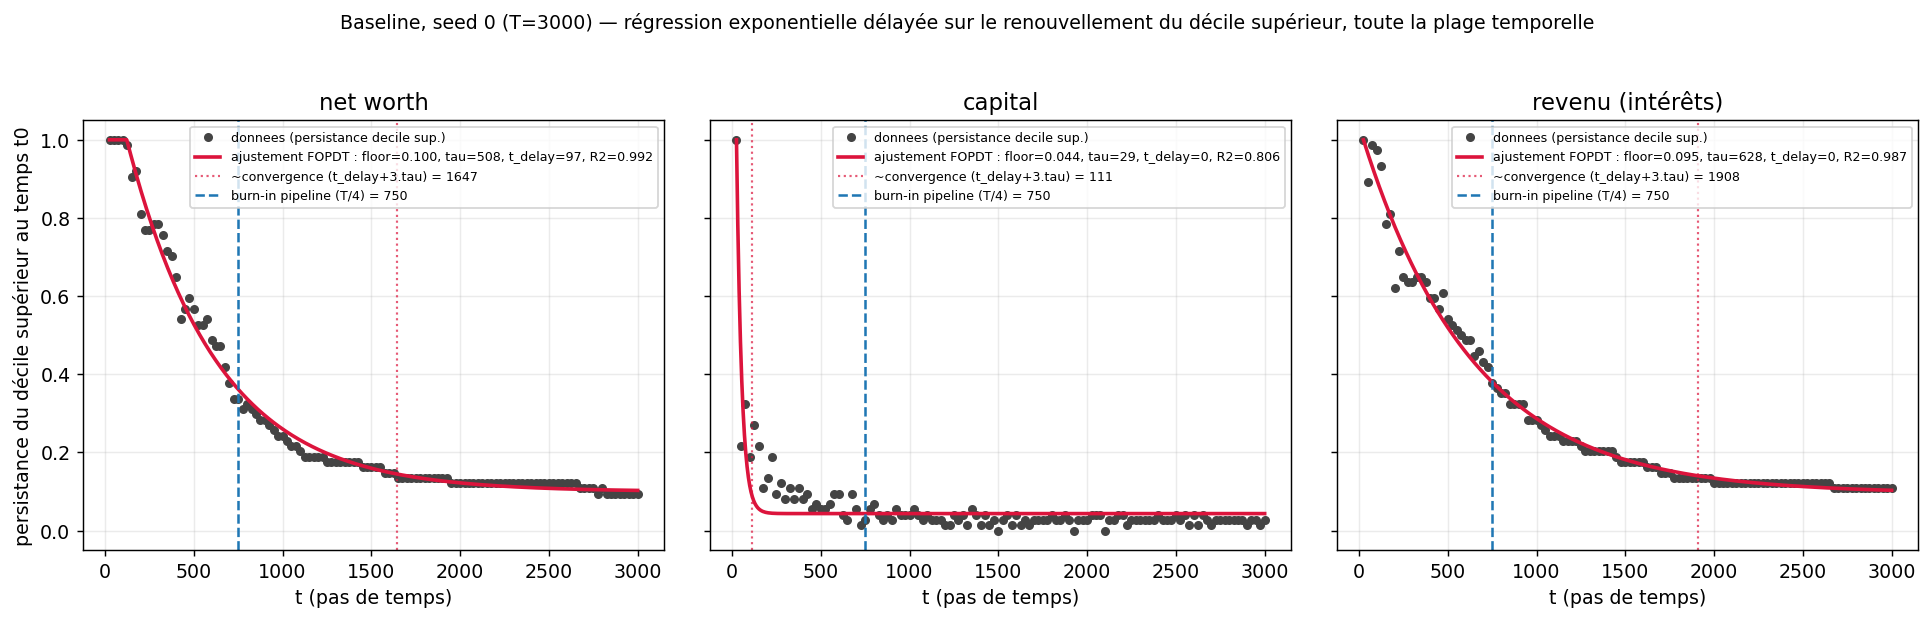
\includegraphics[width=0.95\textwidth]{figures/fig8_renouvellement_fopdt_exemple.png}
\caption{Ajustement sur toute la plage temporelle disponible (pas
seulement la fenêtre de confirmation), baseline graine 0 :
$R^2=0{,}992$ (net worth) et $0{,}987$ (revenu) --- excellent. Le temps
de convergence estimé ($t_{\mathrm{delay}}+3\tau$) est
$\sim$1650--1900 pas, contre un burn-in fixe de 750 ($T/4$) utilisé
jusqu'ici partout dans le pipeline : la fenêtre standard ne couvrait
qu'environ 40\,\% du temps de relaxation réel sur cette cellule. Le
capital ($K$), lui, relaxe quasi instantanément ($\tau\approx 29$) ---
cohérent avec l'homogénéisation rapide déjà documentée.}
\end{figure}

\begin{figure}[H]
\centering
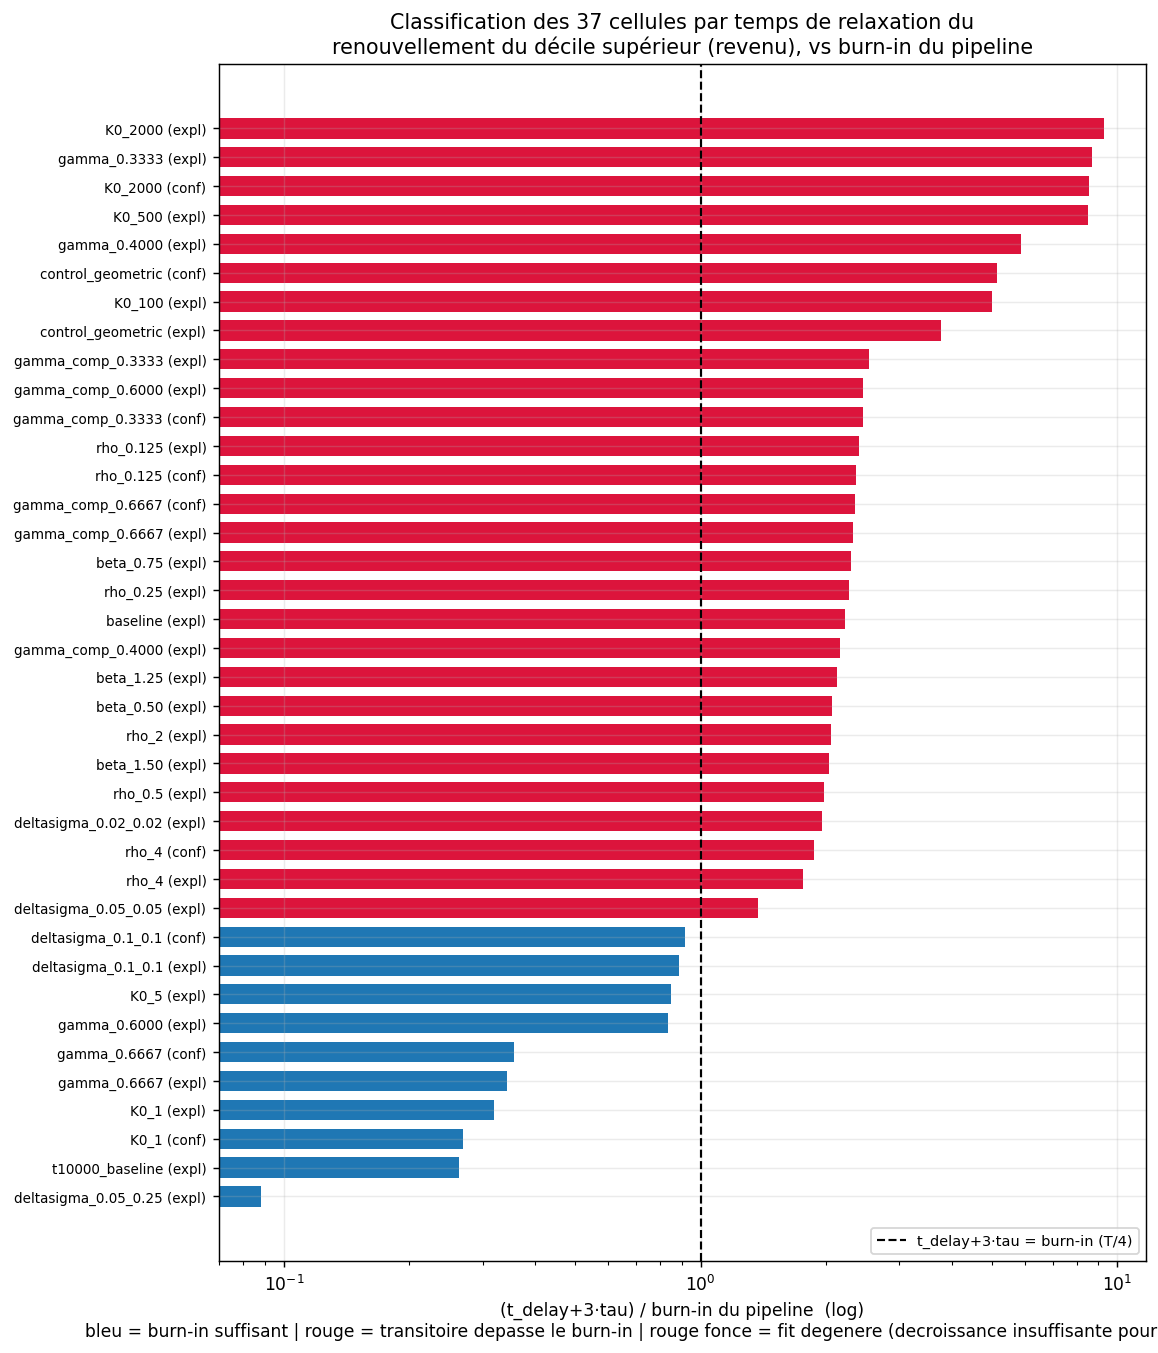
\includegraphics[width=0.85\textwidth]{figures/fig9_classification_relaxation.png}
\caption{Appliqué aux 37 cellules : le capital est toujours rapide (0
problème), mais le revenu d'intérêt et le net worth dépassent le
burn-in standard dans 27 cellules sur 37 --- de peu
(\code{deltasigma\_0.05\_0.05} : $\times 1{,}4$) à massivement
(\code{K0\_2000} : $\times 10$--$11$). C'est ce classement qui définit
les runs « légers » (fenêtre repositionnée après convergence) et
« sévères » (pas de marge, un seul instantané).}
\end{figure}

\subsection*{$\eta$ (le levier le plus systématique)}

\begin{table}[h]
\centering
\begin{tabular}{@{}rrrr@{}}
\toprule
$\rho$ & $\hat\alpha$ (confirmation) & $\hat\tau$ & branchement \\
\midrule
0{,}125 & $4{,}172 \pm 0{,}261$ & 1{,}815 & 0{,}478 \\
1 (baseline, exploration) & $3{,}890 \pm 0{,}020$ & 1{,}412 & 0{,}786 \\
4 & $4{,}130 \pm 0{,}134$ & 0{,}989 & 0{,}891 \\
\bottomrule
\end{tabular}
\end{table}

Effet non monotone (les deux extrêmes ont un $\hat\alpha$ plus élevé que
la baseline), et l'écart-type inter-graines grandit nettement aux
extrêmes ($0{,}26$ à $\rho=0{,}125$, contre $0{,}02$ à la baseline) ---
l'effet reste net mais moins précis qu'à baseline. Le rapport de
branchement, lui, reste parfaitement monotone : $0{,}478 \to 0{,}786
\to 0{,}891$ --- $\eta$ est avant tout un levier sur
l'\textbf{intensité des cascades}, pas seulement sur les intérêts. Le
paramètre $\beta$ ($\eta$ non linéaire) n'a en revanche
\textbf{aucun effet mesurable} : $\hat\alpha$ reste dans
$3{,}80$--$3{,}89$ sur toute la plage testée, barres d'erreur largement
chevauchantes.

\begin{figure}[H]
\centering
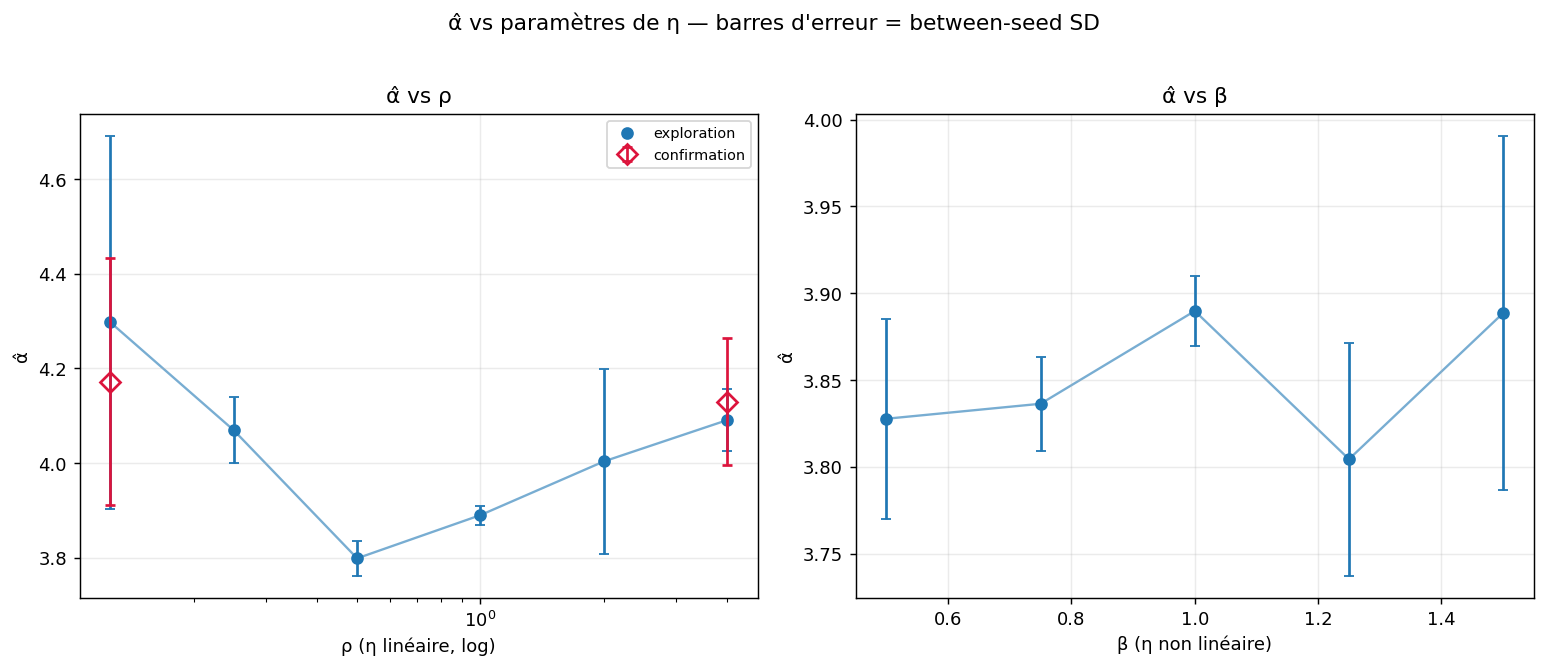
\includegraphics[width=0.95\textwidth]{figures/fig14_alpha_vs_eta.png}
\caption{Panneau gauche : $\hat\alpha$ vs $\rho$, non monotone mais net.
Panneau droit : $\hat\alpha$ vs $\beta$, plat --- aucun effet
distinguable du bruit.}
\end{figure}

\begin{figure}[H]
\centering
\begin{minipage}{0.48\textwidth}
\centering
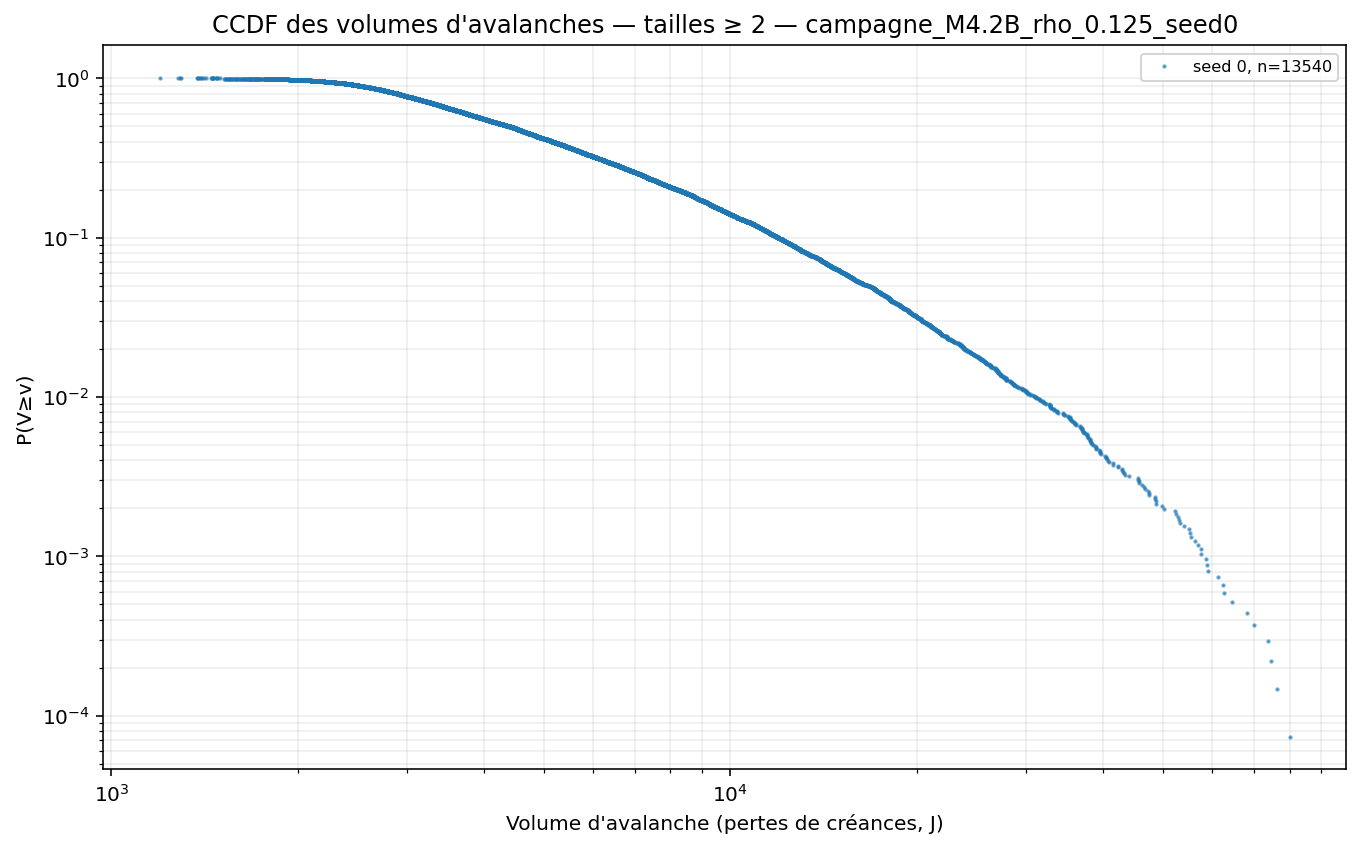
\includegraphics[width=\textwidth]{figures/sim_avalanches_rho_0125.png}
\end{minipage}
\hfill
\begin{minipage}{0.48\textwidth}
\centering
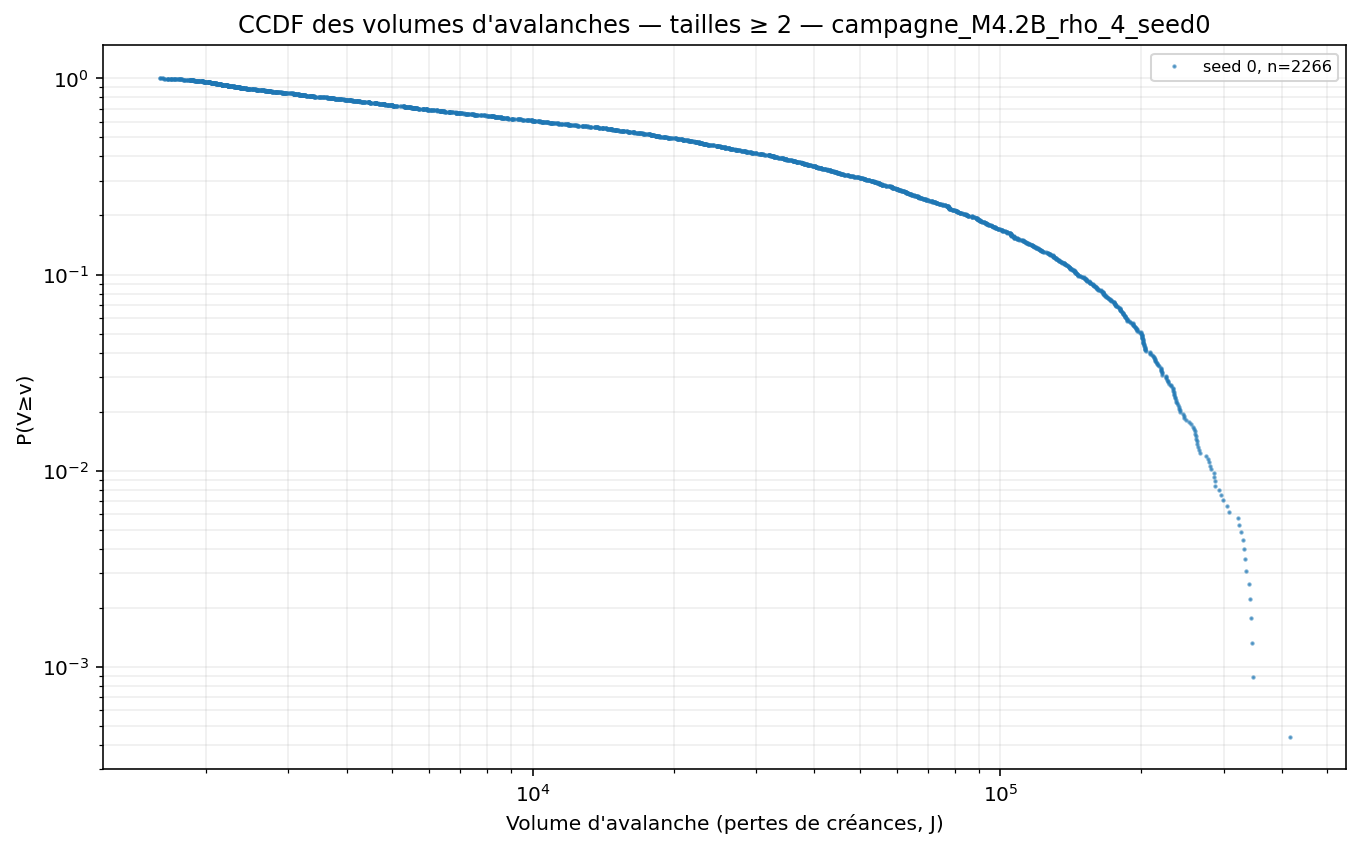
\includegraphics[width=\textwidth]{figures/sim_avalanches_rho_4.png}
\end{minipage}
\caption{CCDF des volumes d'avalanches, $\rho=0{,}125$ (gauche) contre
$\rho=4$ (droite), sorties brutes du moteur (une graine d'exploration
chacune). À gauche, marché clairsemé : les avalanches restent petites
(volume maximal $\approx 5\times10^4$) et la CCDF s'incurve tôt. À
droite, marché dense : les avalanches atteignent des volumes dix fois
plus grands ($\approx 5\times10^5$) sur une pente plus soutenue avant de
s'incurver --- signature visuelle directe d'une dynamique plus critique,
cohérente avec le rapport de branchement plus élevé ($0{,}891$ contre
$0{,}478$).}
\end{figure}

\subsection*{$K_0$ (mécanisme \emph{deg\_out}, effet non simple, deux cellules sévères)}

\begin{table}[h]
\centering
\begin{tabular}{@{}rrrlrr@{}}
\toprule
$K_0$ & $\hat\alpha$ & écart-type & statut & population & plancher renouv. \\
\midrule
1 & 3{,}592 (conf) / 3{,}641 (expl) & 0{,}072 / 0{,}081 & léger & 362--429 & 0{,}000 \\
25 (baseline) & 3{,}890 & 0{,}020 & léger & $\sim$1147 & 0{,}088 \\
100 & 3{,}665 & 0{,}128 & \textbf{sévère} & $\sim$1980 & --- \\
500 & 3{,}266 & 0{,}113 & \textbf{sévère} & $\sim$3850 & --- \\
2000 & 2{,}986 (conf) / 2{,}969 (expl) & 0{,}053 / 0{,}007 & \textbf{sévère} & 7152--7326 & 0{,}796 \\
\bottomrule
\end{tabular}
\end{table}

Effet net et non monotone, confirmé sur graines disjointes aux deux
extrêmes retenus pour confirmation ($K_0=1$, $K_0=2000$). $K_0=100$,
$500$ et $2000$ sont des cellules \textbf{sévères} : un seul instantané
par graine, régime stationnaire non confirmé (\S\ref{sec:criteres}) ---
mais l'estimation elle-même reste très reproductible ($K_0=2000$ :
écart-type inter-graines $0{,}007$ à $0{,}053$, parmi les plus faibles
de toute la campagne). Le changement le plus spectaculaire reste
qualitatif : le plancher de renouvellement de l'élite passe de 0
(turnover total, $K_0=1$) à $0{,}796$ (élite quasi figée, $K_0=2000$).
\textbf{Prudence} : la comparaison $K_0=1$ vs $K_0=2000$ mélange donc un
point bien caractérisé (léger) et un point ponctuel non stationnaire
confirmé (sévère) --- l'écart mesuré ($\sim$0,6) est robuste
statistiquement mais ne doit pas être lu comme deux régimes
stationnaires comparés à égalité.

\begin{figure}[H]
\centering
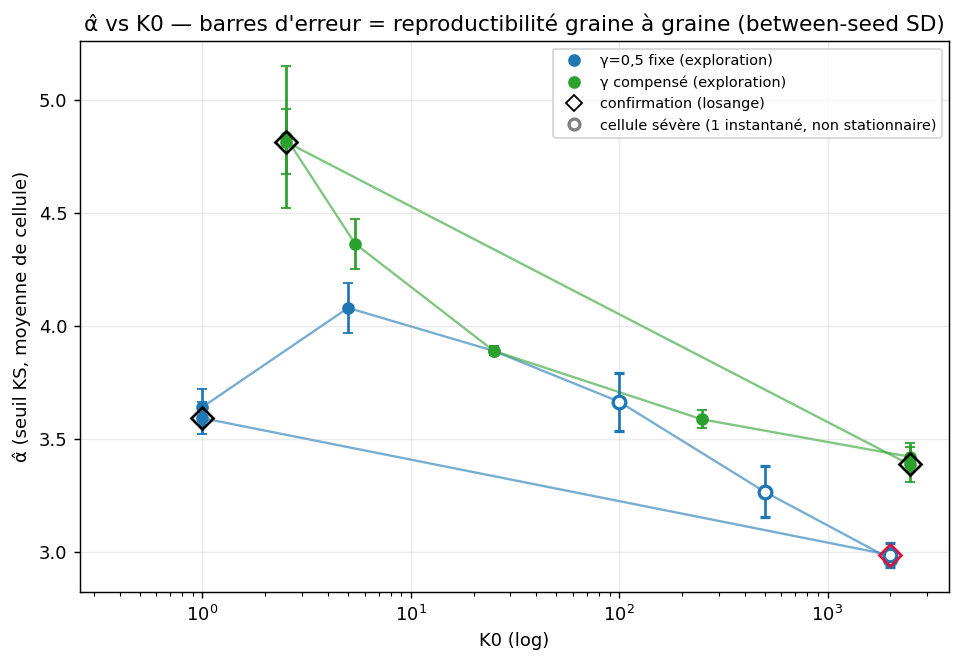
\includegraphics[width=0.85\textwidth]{figures/fig12_alpha_vs_K0.png}
\caption{$\hat\alpha$ vs $K_0$, brut et compensé. Marqueurs creux =
cellules sévères. Losanges = confirmation. Les deux branches ($\gamma=0{,}5$
fixe et $\gamma$ compensé) montrent le même sens d'effet ; l'écart
entre les deux (compensé toujours au-dessus) montre que $\gamma$ et
$K_0$ interagissent plutôt que de se substituer l'un à l'autre.}
\end{figure}

\begin{figure}[H]
\centering
\begin{minipage}{0.48\textwidth}
\centering
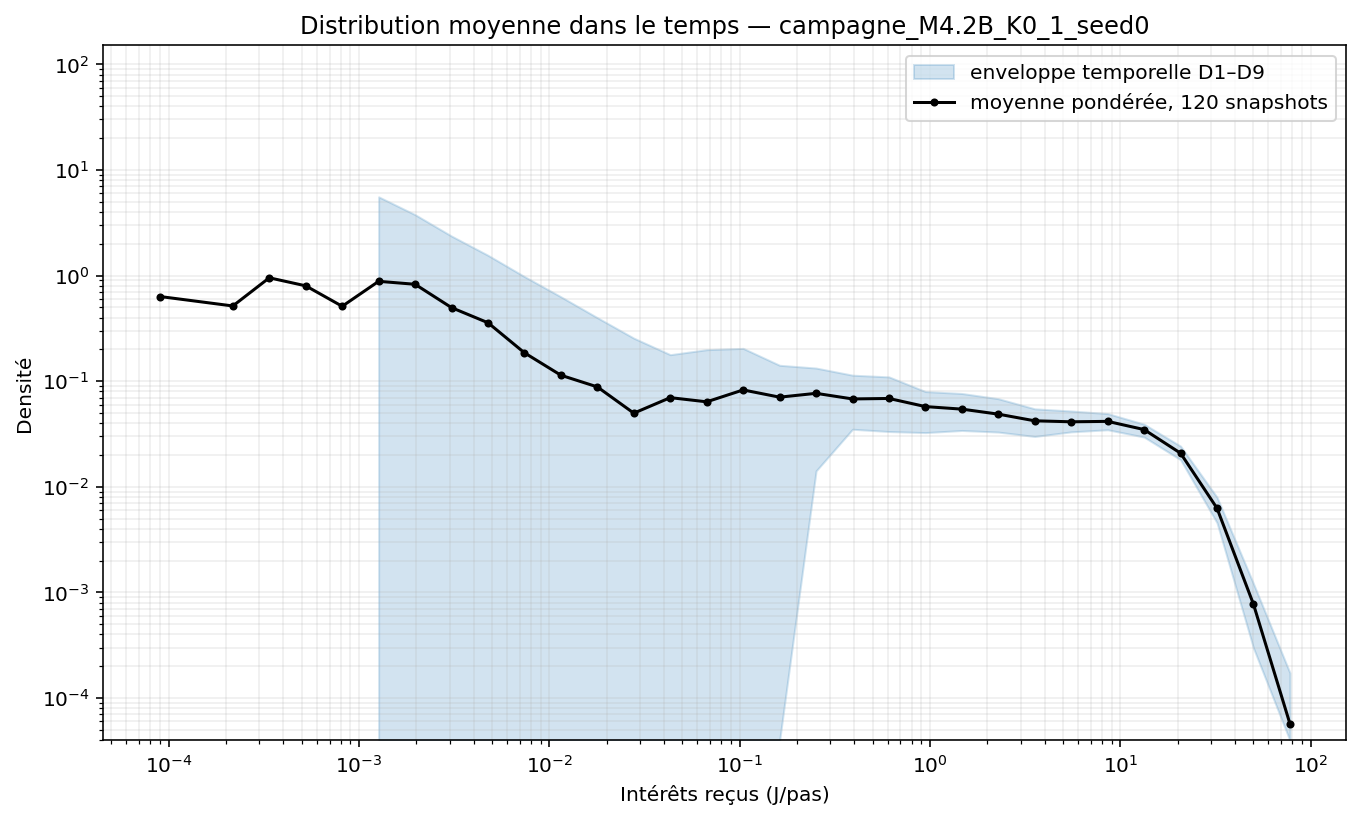
\includegraphics[width=\textwidth]{figures/sim_interets_K0_1.png}
\end{minipage}
\hfill
\begin{minipage}{0.48\textwidth}
\centering
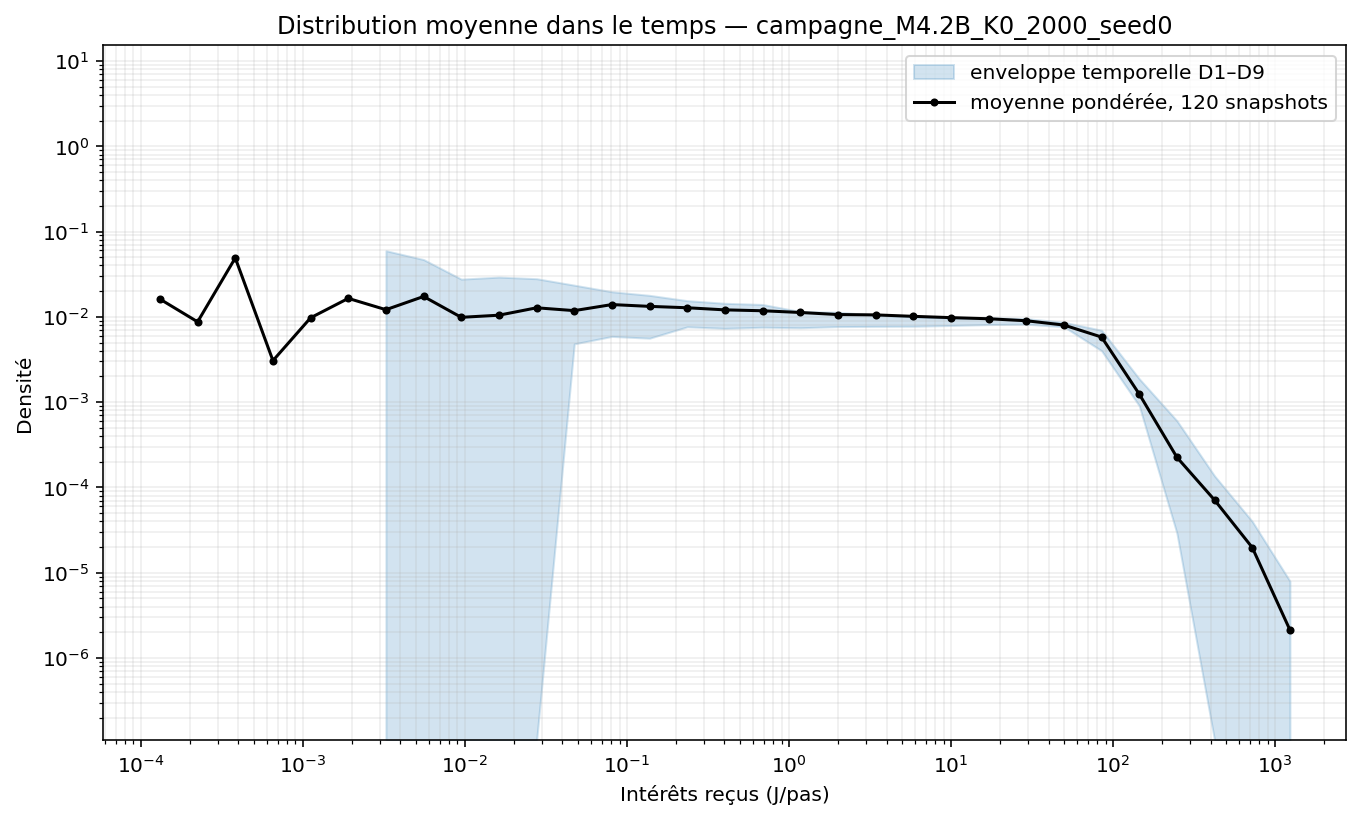
\includegraphics[width=\textwidth]{figures/sim_interets_K0_2000.png}
\end{minipage}
\caption{Distribution des intérêts reçus, $K_0=1$ (gauche) contre
$K_0=2000$ (droite). À $K_0=2000$, la courbe s'étend sur près de 3
décennies de plus en abscisse ($\sim10^3$ J/pas contre $\sim10^2$ à
$K_0=1$) et reste plus haute plus longtemps avant de s'effondrer ---
visuellement plus proche d'une droite en échelle log-log, cohérent avec
le $\hat\alpha$ plus bas mesuré à $K_0=2000$. Rappel : instantané unique
côté $K_0=2000$ (cellule sévère), pas une moyenne sur fenêtre
stationnaire.}
\end{figure}

\begin{figure}[H]
\centering
\begin{minipage}{0.48\textwidth}
\centering
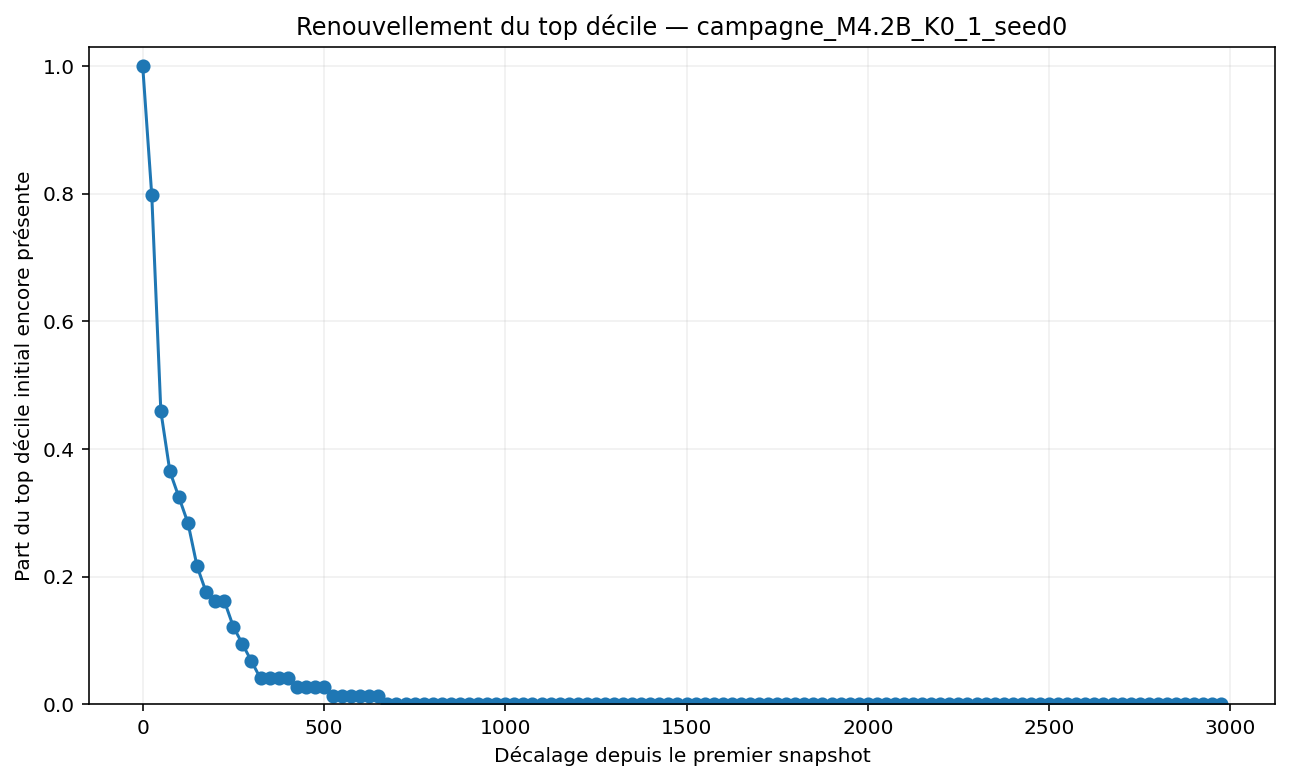
\includegraphics[width=\textwidth]{figures/sim_renouvellement_K0_1.png}
\end{minipage}
\hfill
\begin{minipage}{0.48\textwidth}
\centering
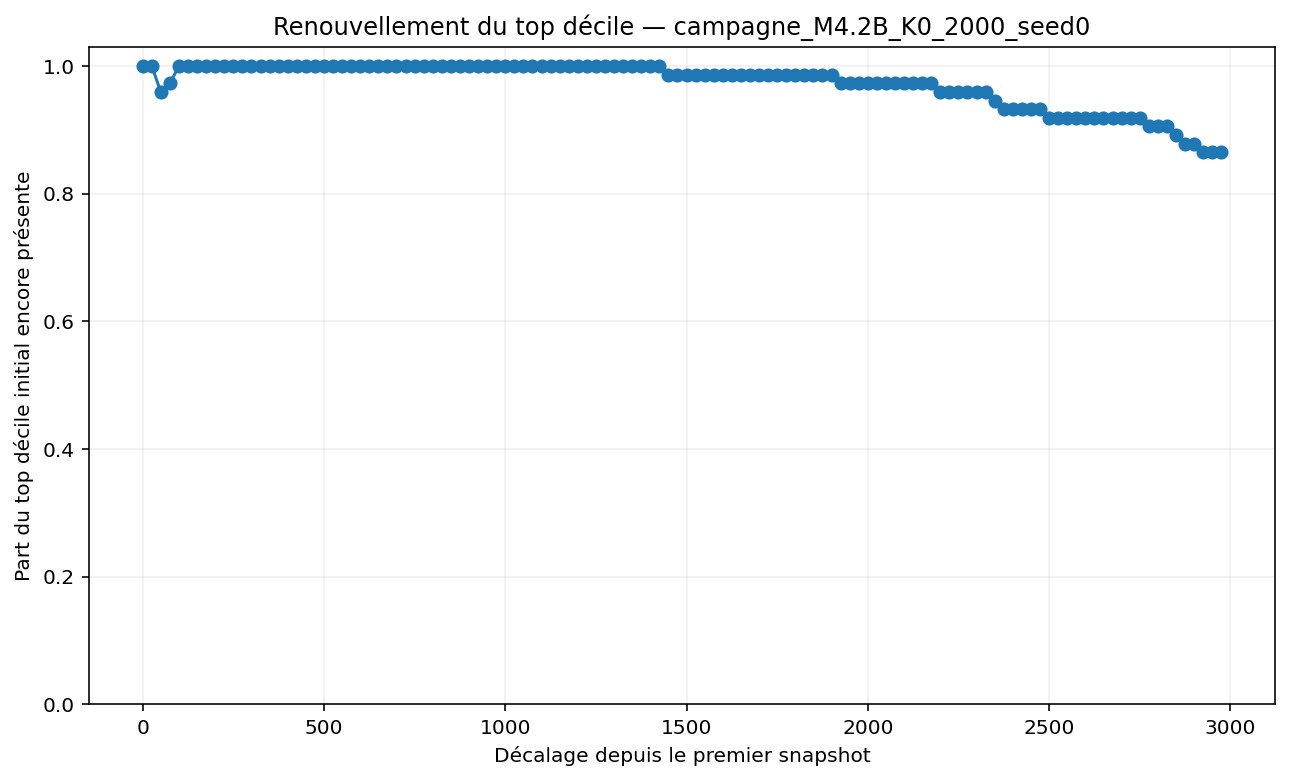
\includegraphics[width=\textwidth]{figures/sim_renouvellement_K0_2000.png}
\end{minipage}
\caption{Renouvellement du top décile, $K_0=1$ (gauche) contre
$K_0=2000$ (droite) --- le contraste le plus spectaculaire de toute la
campagne. À $K_0=1$, l'élite initiale est presque entièrement
renouvelée en moins de 1000 pas. À $K_0=2000$, la même élite reste
identifiable à plus de 85\,\% de sa composition initiale jusqu'à la fin
des 3000 pas simulés --- cohérent avec le diagnostic FOPDT : ce n'est
pas qu'un régime stationnaire tarde à s'installer, la persistance
elle-même reste élevée ($\sim$0,8--0,9) tout du long, un ajustement à
décroissance lente est mal contraint sur des données aussi plates.}
\end{figure}

\subsection*{$\gamma$ (effet réel seulement une fois l'échelle contrôlée)}

\begin{table}[h]
\centering
\begin{tabular}{@{}rll@{}}
\toprule
$\gamma$ & $\hat\alpha$ ($K_0=25$, brut) & $\hat\alpha$ ($K_0$ compensé) \\
\midrule
1/3 & $3{,}793 \pm 0{,}123$ (sévère) & $4{,}835 \pm 0{,}314$ (expl) / $4{,}816 \pm 0{,}143$ (conf) \\
0{,}5 (baseline) & $3{,}890 \pm 0{,}020$ & $3{,}890 \pm 0{,}020$ \\
2/3 & $3{,}374 \pm 0{,}024$ (expl) / $3{,}337 \pm 0{,}031$ (conf) & $3{,}421 \pm 0{,}062$ (expl) / $3{,}387 \pm 0{,}079$ (conf) \\
\bottomrule
\end{tabular}
\end{table}

La branche compensée confirme la décroissance nette observée en
exploration : plus la production est concave ($\gamma$ petit), plus la
queue apparente est lourde ($\hat\alpha$ plus grand). La branche brute
($K_0=25$ fixe) est nettement plus plate --- confondue avec l'effet
d'échelle de $K_0$ tant que $K_0/\Kaut$ n'est pas tenu constant. C'est
le signal le plus propre de toute la campagne pour un paramètre autre
que $\eta$, confirmé sur graines disjointes aux deux extrêmes
compensés.

\begin{figure}[H]
\centering
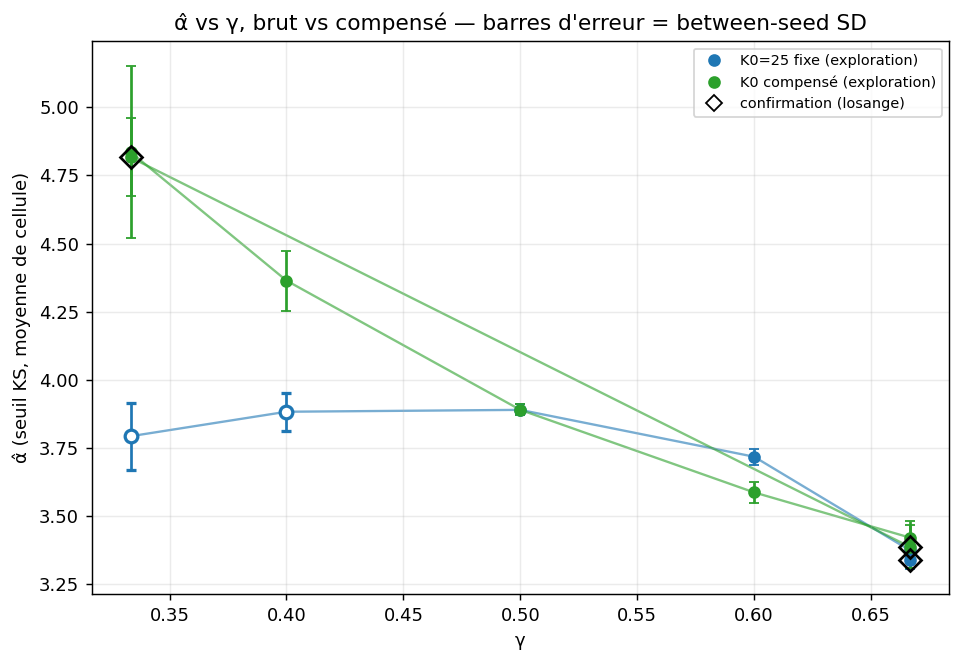
\includegraphics[width=0.72\textwidth]{figures/fig13_alpha_vs_gamma.png}
\caption{$\hat\alpha$ vs $\gamma$, brut vs.\ compensé. La ligne bleue
($K_0$ fixe) est quasi plate ; la ligne verte ($K_0$ compensé) décroît
nettement. Les deux se rejoignent à $\gamma=0{,}5$ par construction
(baseline commune). Losanges = confirmation.}
\end{figure}

\subsection*{$\delta$, $\sigma$ conjoints}

\code{deltasigma\_0.1\_0.1} ($\delta=\sigma=0{,}10$) confirme le signal
exploratoire : $\hat\alpha = 3{,}054 \pm 0{,}035$ (confirmation) /
$3{,}042 \pm 0{,}010$ (exploration), contre $3{,}890$ à baseline --- la
valeur la plus basse de tout le balayage $\delta=\sigma$ conjoint
($0{,}01\to0{,}10$, monotone décroissant), tandis que le rapport de
branchement s'effondre en parallèle à $0{,}386$ (contre $0{,}786$ en
baseline). Un point hors de ce sweep conjoint ($\delta=0{,}05$ fixe,
$\sigma=0{,}25$ seul, réglage historique M4.2) donne au contraire
$\hat\alpha=4{,}382 \pm 0{,}061$ : $\delta$ et $\sigma$ ne poussent donc
pas dans le même sens quand on les sépare, seul leur mouvement
\textbf{conjoint} fait décroître $\hat\alpha$. La direction du
compromis ($\hat\alpha$ plus bas, criticité des avalanches plus basse)
reste la même que celle documentée en exploration, maintenant confirmée
sur graines disjointes.

\begin{figure}[H]
\centering
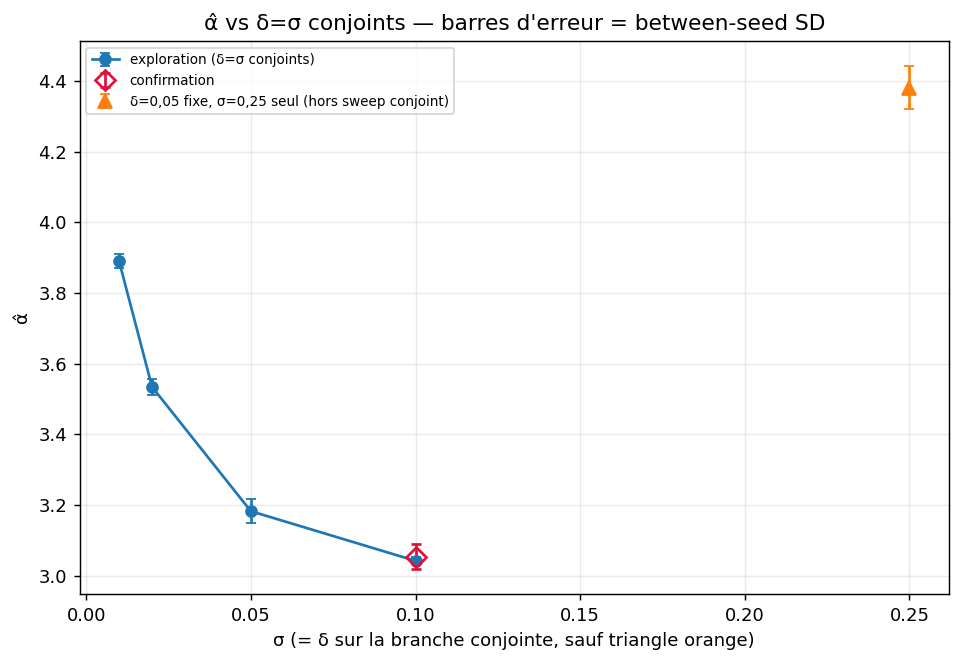
\includegraphics[width=0.72\textwidth]{figures/fig15_alpha_vs_deltasigma.png}
\caption{$\hat\alpha$ vs $\delta=\sigma$ conjoints. La branche bleue
($\delta=\sigma$, sweep conjoint) décroît nettement ; le triangle orange
($\delta=0{,}05$ fixe, $\sigma=0{,}25$ seul) sort de cette tendance ---
preuve directe que ce n'est pas $\sigma$ seul qui pilote l'effet.}
\end{figure}

\section{Réponses aux 17 questions du cahier des charges}

\begin{enumerate}
\item \textbf{Que change la cible arithmétique par rapport à la cible
  géométrique ?} Le principal des deux parties est ramené exactement à
  leur moyenne (contre la moyenne géométrique en M4.2), avec un
  principal non borné plus élevé pour les paires très inégales. À
  baseline autrement identique, la cible arithmétique donne une queue
  apparente plus légère que la cible géométrique : $\hat\alpha=3{,}890
  \pm 0{,}020$ (arithmétique) contre $\hat\alpha=3{,}318 \pm 0{,}113$
  (géométrique, \code{control\_geometric}, \textbf{cellule sévère} ---
  un seul instantané par graine, régime stationnaire non confirmé) ---
  même sens qu'en exploration, confirmé sur graines disjointes malgré la
  réserve sur la cellule géométrique. \fait{} (confirmé), sous
  l'hypothèse Pareto désormais posée au \S\ref{sec:criteres}.

\item \textbf{Quelle est la forme du corps de la distribution
  instantanée des intérêts ?} GB2 (famille à 4 paramètres) gagne
  systématiquement par AIC sur les instantanés testés en phase pilote ;
  l'exponentielle/Weibull restent très compétitifs à 1-2 paramètres.
  \fait{} phase pilote uniquement --- non re-testé systématiquement sur
  les 9 cellules de confirmation.

\item \textbf{Existe-t-il une queue Pareto robuste des intérêts ? Dans
  quelles régions du modèle ?} \textbf{La question n'a pas pu être
  tranchée, dans aucun sens.} Trois versions successives d'un test
  d'existence ont été essayées (\S\ref{sec:criteres}) ; la dernière
  (facteur d'admissibilité continu, bootstrap, 132 runs) donne
  $A<0{,}5$ partout, mais la décomposition montre que c'est presque
  entièrement un problème de \textbf{volume de données dans la queue
  extrême} (couverture médiane $0{,}22$), pas une preuve de courbure
  (platitude médiane $0{,}56$, correcte là où elle est mesurable). Ce
  n'est donc ni « oui, robuste » ni « non, clairement pas Pareto » :
  c'est \textbf{non testable avec les données de ce programme}.
  Décision prise en conséquence (\S\ref{sec:criteres}) : l'existence est
  posée comme hypothèse de travail, et ce rapport caractérise
  $\hat\alpha$ sous cette hypothèse plutôt que de continuer à chercher à
  trancher l'existence elle-même.

\item \textbf{Quelle famille globale ou composite décrit le mieux la
  distribution ?} GB2 pour le corps (Q2) ; aucune composite à raccord
  Pareto explicite n'apporte quoi que ce soit par rapport à GB2/mélange
  lognormal en phase pilote. \fait{} phase pilote uniquement.

\item \textbf{Quel est le domaine accessible des exposants de queue des
  intérêts ?} $\hat\alpha$ (moyenne de cellule, seuil KS, sous
  l'hypothèse Pareto posée au \S\ref{sec:criteres}) varie de
  \textbf{2,969--2,986} ($K_0=2000$, exploration/confirmation, cellule
  sévère) à \textbf{4,816--4,835} (\code{gamma\_comp\_0.3333}) --- un
  facteur $\sim$1,6. \textbf{Attention} : l'existence même de la loi de
  puissance n'étant pas établie (Q3), ce ne sont pas des exposants
  Pareto démontrés, mais des ajustements reproductibles graine à graine
  (écart-type inter-graines médian $0{,}070$) sous l'hypothèse de
  travail. \fait{} avec cette réserve.

\item \textbf{Quels paramètres contrôlent principalement cette queue
  (apparente) ?} $\eta$ (effet le plus systématique, non monotone, sur
  $\hat\alpha$ ET sur le rapport de branchement), $\gamma$ une fois
  l'échelle contrôlée (effet le plus propre et monotone), $K_0$ (effet
  fort mais non monotone, deux cellules sévères aux extrêmes hauts),
  $\delta/\sigma$ conjoints (effet monotone marqué sur $\hat\alpha$,
  avec effondrement parallèle du rapport de branchement). $\beta$
  ($\eta$ non linéaire) n'a aucun effet mesurable. \fait{}

\item \textbf{Quel rôle spécifique joue $\eta$ ?} Le levier le plus
  systématique du grid : contrôle $\hat\alpha$ (effet non monotone mais
  net, $3{,}89\to4{,}17$--$4{,}30$ aux extrêmes) et --- de façon
  parfaitement monotone --- $\hat\tau$ et le rapport de branchement
  ($0{,}478$ à $\rho=0{,}125$ $\to$ $0{,}786$ à baseline $\to$
  $0{,}891$ à $\rho=4$). \fait{} confirmé sur graines disjointes.

\item \textbf{Quel rôle jouent $K_0$, $\gamma$, $\lambda$, $\delta$ et
  $\sigma$ ?} $K_0$ : mécanisme \emph{deg\_out}, effet dominant sur la
  mobilité sociale de long terme (plancher de renouvellement
  $0{,}000\to0{,}796$), effet non monotone sur $\hat\alpha$, deux
  cellules sévères aux extrêmes hauts (régime stationnaire non
  confirmé). $\gamma$ : confondu avec l'échelle sauf compensation
  $K_0/\Kaut$ ; une fois compensé, effet propre et monotone
  ($\hat\alpha$ $3{,}89\to4{,}82$ quand $\gamma$ diminue). $\delta$,
  $\sigma$ : effet monotone marqué sur $\hat\alpha$
  ($3{,}89\to3{,}04$ sur le sweep conjoint), en parallèle d'un
  effondrement de la criticalité des avalanches --- mais
  $\delta=0{,}05,\sigma=0{,}25$ seul (hors sweep conjoint) donne un
  effet opposé ($\hat\alpha=4{,}38$), donc ce n'est pas $\sigma$ seul
  qui pilote. $\lambda$ : non re-testé (fixé à 30) ; seule évidence, le
  balayage du pilote ($\lambda \in \{10;30;100\}$), qui montre une
  dérive de $\hat\tau$ et un estimateur de coupure saturé à
  $\lambda=100$. \incertitude{} sur le rôle de $\lambda$ au-delà du
  pilote.

\item \textbf{Quel rôle jouent respectivement $r$, $q$ et $rq$ ?}
  Mécanisme établi en pilote : $r$ quasi constant, dispersion du
  log-revenu dominée à 77\,\% par le nombre de contrats accumulés
  (\emph{deg\_out}), 23\,\% par $rq$ moyen. Les écarts de la part
  \emph{deg\_out} par rapport à la baseline, mesurés sur les 9 cellules
  de confirmation, vont de $-0{,}17$ (\code{rho\_0.125},
  \code{gamma\_0.6667}, \code{deltasigma\_0.1\_0.1}) à $+0{,}07$
  (\code{control\_geometric}) --- le mécanisme quantité/prix reste actif
  sur un ensemble de cellules bien plus large qu'en pilote. \fait{}
  confirmé plus largement.

\item \textbf{La règle de taux géométrique produit-elle des effets
  pathologiques ?} Non au sens service : 0 défaut de liquidité observé
  en pilote. Oui au sens levier : un service $c=rq$ tel que
  $c/F_\gamma(K_b')\approx1{,}57$ dès la création du contrat pour
  certaines paires, résolu en faillite différée, jamais en défaut de
  service immédiat. \fait{} phase pilote uniquement.

\item \textbf{Les avalanches conservent-elles une structure en loi de
  puissance dans les mêmes régimes ?} Descriptivement oui : sur les 9
  cellules de confirmation, le rapport de branchement reste non nul et
  varie de façon interprétable ($0{,}386$ à $0{,}891$). Mais
  l'\textbf{indépendance de taille} de $\hat\tau$ n'est pas établie et
  n'est pas testable avec la conception actuelle de la confirmation
  (\S\ref{sec:limites}). \fait{} (persistance) + \incertitude{}
  (indépendance de taille).

\item \textbf{Existe-t-il un compromis entre la queue des revenus et la
  criticalité des cascades ?} Oui, clairement, sur la branche
  $\delta/\sigma$ : la valeur la plus basse de $\hat\alpha$ de tout le
  sweep conjoint (\code{deltasigma\_0.1\_0.1}, $\hat\alpha\approx3{,}05$)
  est aussi celle où le rapport de branchement s'effondre le plus
  ($0{,}786 \to 0{,}386$). \fait{} confirmé sur graines disjointes.

\item \textbf{Quel domaine de paramètres satisfait simultanément les
  deux objectifs ?} Question désormais mal posée telle quelle :
  l'objectif A n'a pu être ni établi ni infirmé au sens strict (Q3),
  donc « satisfaire l'objectif A » n'a pas de réponse binaire. Sous
  l'hypothèse Pareto (\S\ref{sec:criteres}), aucune des 9 cellules de
  confirmation ne combine un déplacement notable de $\hat\alpha$ ET un
  rapport de branchement préservé proche de la baseline ($0{,}786$) ---
  le seul mouvement net sur $\hat\alpha$ dans le sens d'une queue plus
  légère ($\delta=\sigma$) coûte systématiquement en criticalité des
  avalanches. \fait{} (sous l'hypothèse Pareto), la question au sens
  strict du protocole restant \textbf{non tranchable}.

\item \textbf{Les effets survivent-ils aux graines, au temps et à la
  taille du système ?} Graines : oui, très bien --- écart-type
  inter-graines médian $0{,}070$ sur les cellules de confirmation
  (\S\ref{sec:criteres}--\ref{sec:resultat}), nettement plus petit que
  l'écart-type intra-instantané (médian $0{,}341$) : la moyenne de
  cellule est reproductible même quand un instantané isolé serait
  bruité. Temps : la cellule à $T=10000$ reste dans la même gamme de
  $\hat\alpha$ que $T=3000$. Taille : non testable avec la conception
  actuelle (Q11). \incertitude{}

\item \textbf{Quels changements observés relèvent d'un exposant, d'une
  coupure, d'une échelle, d'une masse en zéro ou d'un transitoire ?} Un
  « coude » après la cassure est présent dans toutes les simulations de
  ce programme (confirmé visuellement, \S\ref{sec:reperes}) --- la
  question de savoir s'il s'agit d'une coupure franche (pas d'exposant
  Pareto authentique) ou d'une vraie queue de puissance affectée par un
  manque de données dans l'extrême n'a \textbf{pas pu être tranchée}
  avec le volume de données disponible (Q3, \S\ref{sec:criteres}) : les
  trois tentatives de test successives (seuil/2, seuil$\times$2, facteur
  d'admissibilité continu) échouent toutes par manque de points dans la
  queue extrême, pas par preuve claire de courbure. \incertitude{} ---
  position retenue : traiter l'existence comme hypothèse et caractériser
  $\hat\alpha$ dans la région testable, en gardant explicitement cette
  réserve à chaque valeur citée.

\item \textbf{Si une refonte du modèle a été nécessaire, quelle
  hypothèse la justifie et quelle ablation démontre son effet ?} Aucune
  refonte des mécanismes n'a été effectuée. La seule modification
  constitutive est la cible arithmétique elle-même, déjà spécifiée par
  le programme et vérifiée par parité stricte avec M4.2 (écart flottant
  $0{,}000\mathrm{e}{+00}$ dans les régimes communs). Non applicable /
  non fait, hors périmètre du temps disponible.

\item \textbf{Quels éléments restent incertains ?} Voir
  \S\ref{sec:limites} pour la liste complète et sourcée.
\end{enumerate}

\section{Limites et non testé}
\label{sec:limites}

\begin{itemize}
\item \textbf{Indépendance de taille des avalanches (objectif B, critère
  formel)} : non établie et non testable avec la conception actuelle de
  la confirmation. Les 9 cellules ont toutes $\lambda=30$ fixe ; $K_0$
  varie fortement la taille de population mais change simultanément
  l'inégalité (Gini $\times 8$), la mobilité (plancher de renouvellement
  $0{,}000 \to 0{,}796$) et le mécanisme de prix ($\Delta$
  \code{share\_mean\_rq} jusqu'à $0{,}24$) --- ce n'est pas « à
  paramètres autrement identiques » au sens du protocole. La seule
  évidence disponible dans tout le programme est le balayage
  $\lambda \in \{10;30;100\}$ du pilote (une seule graine) : $\hat\tau$
  dérive de $1{,}19$-$1{,}27$ à $1{,}75$, et l'estimateur de coupure
  sature à sa borne numérique à $\lambda=100$ (aucune coupure finie
  détectée). Conclusion du pilote reconduite ici sans changement :
  \textbf{aucun exposant d'avalanche indépendant de la taille n'a été
  établi dans ce programme}.
\item \textbf{Forme du corps de la distribution (GB2 et alternatives),
  Q2/Q4} : établie en phase pilote sur un petit nombre d'instantanés,
  jamais re-testée systématiquement sur les 87 runs d'exploration ni les
  45 de confirmation.
\item \textbf{Rôle de $\lambda$ (Q8)} : au-delà du balayage pilote à une
  graine, non re-testé --- $\lambda=30$ fixe sur toute l'exploration et
  la confirmation.
\item \textbf{Pathologie de la règle de taux (Q10)} : vérifiée en pilote
  uniquement (0 défaut de liquidité) ; \code{book\_errors} est collecté
  par run dans \code{analysis.json} mais n'a pas été systématiquement
  agrégé sur les 132 runs exploration+confirmation pour ce rapport.
\item \textbf{Refonte de mécanisme (Q16)} : non tentée, faute de temps
  --- le prompt complet l'autorise en second recours ; sa nécessité est
  d'autant moins évidente maintenant que l'objectif A n'a pu être ni
  établi ni infirmé (Q3, Q15) plutôt que clairement réfuté.
\item \textbf{\code{gamma\_comp\_0.3333}} : la valeur de $\hat\alpha$ la
  plus élevée de toute la campagne ($4{,}82$--$4{,}84$) ; le mécanisme
  précis n'a pas été creusé au-delà de la décomposition
  \emph{deg\_out}/$rq$ déjà rapportée (Q9).
\item \textbf{Test d'existence abandonné, pas résolu
  (\S\ref{sec:criteres})} : les trois versions successives du critère 1
  (seuil/2, seuil$\times$2, facteur d'admissibilité continu) ont toutes
  échoué à trancher, pour des raisons différentes --- ce n'est pas une
  preuve que la queue de Pareto n'existe pas, c'est une limite de
  puissance statistique de ce programme (populations et fenêtres
  temporelles simulées). Un programme futur avec des populations plus
  grandes et/ou des fenêtres plus longues pourrait rendre ce test à
  nouveau calculable.
\item \textbf{Bootstrap intra-instantané} : rééchantillonne le snapshot
  lui-même (avec remise) ; suppose implicitement les observations
  intra-instantané indépendantes, ce qui n'est vrai qu'approximativement
  (les entités partagent une structure de réseau au même instant). Le
  seuil KS est re-sélectionné à chaque tirage (choix demandé
  explicitement) mais aucune correction de dépendance réseau n'est
  appliquée au-delà de ça.
\item \textbf{Espacement des instantanés par $\tau$ (fenêtre « légère »)} :
  l'hypothèse que les instantanés espacés d'au moins un temps
  caractéristique $\tau$ (mesuré sur le \emph{renouvellement}) sont
  approximativement décorrélés pour la statistique de \emph{queue des
  intérêts} est une approximation raisonnable, pas une mesure directe du
  temps d'autocorrélation de $\hat\alpha$ lui-même --- non vérifiée
  indépendamment.
\item \textbf{Cellules sévères} (\code{K0\_100}, \code{K0\_500},
  \code{K0\_2000}, \code{control\_geometric}) : un seul instantané par
  graine, aucune dispersion inter-instantanés calculable, régime
  stationnaire non confirmé. Les valeurs de $\hat\alpha$ rapportées pour
  ces cellules sont reproductibles graine à graine (écart-type
  inter-graines souvent $<0{,}1$) mais ne doivent pas être lues comme
  des moyennes de régime établi.
\end{itemize}

\section*{À ne pas oublier en citant ce rapport}

Le résultat central (\S\ref{sec:criteres}, \S\ref{sec:resultat}, Q3) est
un \textbf{résultat honnête sur les limites de ce qui est démontrable
avec ce volume de données}, pas un échec de calcul ni une limite de
temps : trois versions successives d'un test d'existence de la queue de
Pareto ont été tentées, à trois échelles de preuve croissantes (pilote
$\to$ exploration $\to$ confirmation à graines disjointes), et aucune
n'a pu trancher --- la dernière (facteur d'admissibilité continu,
bootstrap) montre que c'est presque partout un problème de
\textbf{volume de données dans la queue extrême} (couverture médiane
$0{,}22$ sur l'échelle testée), pas une preuve de courbure (platitude
correcte là où mesurable). \textbf{L'existence de la queue de Pareto est
donc posée comme hypothèse de travail} (décision du 6 août 2026,
\S\ref{sec:criteres}), en reconnaissant explicitement le « coude »
présent après la cassure dans toutes les simulations. Sous cette
hypothèse, $\hat\alpha$ est mesurable, reproductible d'une graine à
l'autre (écart-type inter-graines médian $0{,}070$, très inférieur à
l'écart-type intra-instantané médian $0{,}341$), et répond de façon
interprétable aux paramètres testés (\S\ref{sec:parametres}) --- c'est
ce résultat, positif et quantitatif, qui constitue l'apport substantiel
de ce rapport, à distinguer clairement de la question (non tranchée) de
l'existence elle-même.

\end{document}
